%!TEX root = ../../thesis.tex
\section{Exact Real Arithmetic}\label{sec:exact real arithmetic}
	Using interval arithmetic or arbitrary precision arithmetic, 
	the precision is set in the beginning and rounding and truncation errors still accumulate.
	Without previous careful analysis, there is no guarantee that the result's
  precision will suffice.

	In contrast, the goal of exact real arithmetic is to perform computations on real numbers without 
	accumulating errors.
  
  In practice, that means that on demand a number can be printed up to any desired precision. 
	More precisely, the user does not specify the precision the numbers are represented with in the beginning,
	but gives a desired precision \textbf{for the answer} of the computation.
  
  The implementation has to take care of the steps necessary to achieve the
  precision.
  For the user, it should seem like real numbers are manipulated exactly, while
  of course internally the implementation still works on finite approximations.

	There are several approaches to exact real arithmetic.
	For example
  \begin{enumerate}
      \item \textbf{Signed-digit Streams}: A real number is represented as an infinite
       string stream. This is very close to the definition with type-2
       machines.
     \item \textbf{Continued Fractions}: A real number is represented by its continued
       fraction representation. Rational numbers have a finite representation,
       while irrational numbers have an infinite representation.
     \item \textbf{Directed Acyclic Graphs (DAGs)}: A real number is given by an
       algorithm that computes an approximation to the number with a desired
       error bound. Arithmetic expressions are expressed as graphs with real
       number leaves.
  \end{enumerate}
  Since the approach followed in this thesis is the DAG approach, it is the
  only one that will be described in more detail.
	\subsection{DAGs}
  \begin{figure}[h]
      \centering
      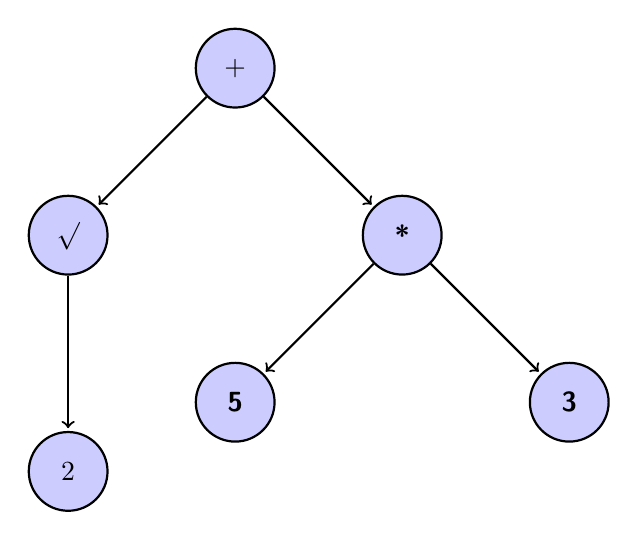
\begin{tikzpicture}[->,shorten >=1pt,auto,node distance=3cm,
  thick,minimum size=1cm,main node/.style={circle,fill=blue!20,draw,font=\sffamily\bfseries}]

  \node[main node] (1) {$+$};
  \node[main node] (2) [below left of=1] {$\sqrt{}$};
  \node[main node] (6) [below of=2] {$2$};
  \node[main node] (3) [below right of=1] {*};
  \node[main node] (4) [below left of=3] {5};
  \node[main node] (5) [below right of=3] {3};

  \path[every node/.style={font=\sffamily\small}]
  (1) edge (2)
  (2) edge (6)
  (1) edge (3)
  (3) edge (4)
  (3) edge (5);
\end{tikzpicture}
\caption{The DAG representation for the expression $\sqrt 2+(2 + 5*3)$}
    \end{figure}
		An arithmetic expression over real numbers can be expressed by a directed acyclic graph (DAG)
		where the leaf nodes are real numbers and the inner nodes are operations on real numbers.
		
    The inner nodes contain the information how precise the inputs to the
    operation have to be to guarantee a given output precision.
    Thus, the needed precision can be propagated down to the leaf nodes, and
    the algorithms to approximate the real numbers can be invoked.

    The term \textbf{evaluating} is used to describe the process of getting an approximation
    to the real number represented by a DAG with a desired output  precision.

		There are essentially two ways to evaluate a DAG:
		\begin{enumerate}
			\item \textbf{Top-down evaluation}: The desired precision is computed from the top node down to the leaves.
			That is, a node contains the information how precisely it needs the
      input given by its children to compute the output with the necessary precision.
      The top node is given the desired output precision, and it then asks its
      children to provide this input.
			\item \textbf{Bottom-up evaluation}:  the computation is started with a fixed precision in the leaf nodes. 
			It is kept track of the errors when going upward in the DAG (this can
      be done e.g. by using interval arithmetic). 
			At the top the error bound is compared to the desired output precision. 
      If the error is too large, the computation is restarted with higher
      precision.
		\end{enumerate}
    \begin{figure}[h]
      \centering
      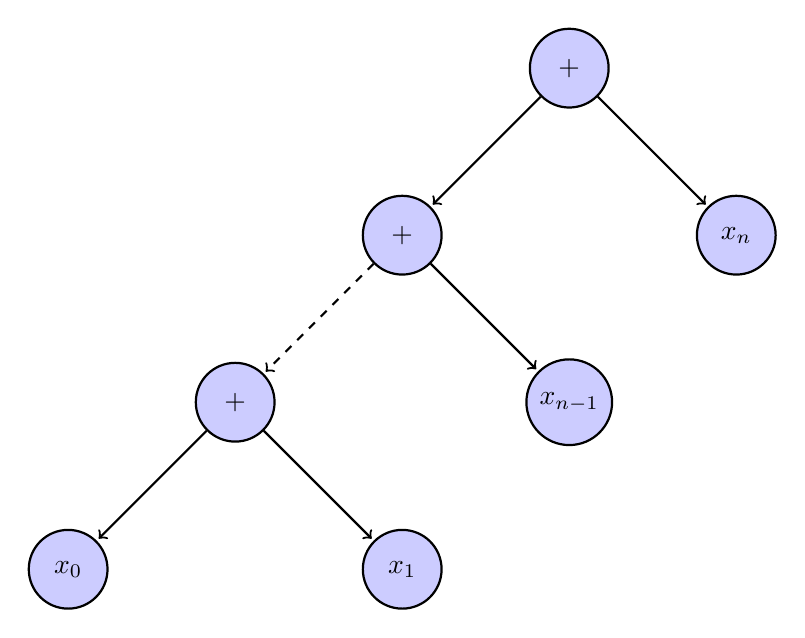
\begin{tikzpicture}[->,shorten >=1pt,auto,node distance=3cm,minimum
          size=1cm,thick,main node/.style={circle,fill=blue!20,draw,font=\sffamily\bfseries}]

  \node[main node] (1) {$+$};
  \node[main node] (2) [below left of=1] {$x_0$};
  \node[main node] (3) [below right of=1] {$x_1$};
  \node[main node] (4) [above right of=1] {$+$};
  \node[main node] (5) [below right of=4] {$x_{n-1}$};
  \node[main node] (6) [above right of=4] {$+$};
  \node[main node] (7) [below right of=6] {$x_n$};
  \path[every node/.style={font=\sffamily\small}]
  (1) edge (2)
  (1) edge (3)
  (4) edge (5)
  (6) edge (4)
  (6) edge (7);
  \path[every node/.style={font=\sffamily\small}]
  (4) edge (1) [dashed] ;
\end{tikzpicture}
\caption{The DAG created when the expression $\sum_{i=0}^n x_i$ is computed
iteratively}\label{fig:sum dag}
\end{figure}
		While the top-down approach seems to evade unnecessary recomputations, the
    precision needed is usually largely overestimated.

    For example, to compute additions of two numbers up to precision $2^{-n}$,
    it suffices to have the inputs with precision $2^{-(n+1)}$.
    Now, if the sum $x := \sum_{i=0}^(1000) x_i$ is computed iteratively (e.g. in a
    for-loop), a DAG as in Figure \ref{fig:sum dag} will be created. 
    Thus, $x_0$ has to be computed with precision $2^{-(n+1000)}$ while actually
    computing all input values with error less than $2^{-(n+10)}$ would 
    suffice to guarantee error of the sum of less than $2^{-n}$.
    This makes the bottom-up approach more feasible in many cases.

    In general, the DAG approach has the problem, that saving the DAG needs a
    huge amount of memory.
    Arithmetic operations in loops, that are executed many times, quickly grow
    the created DAG and thus may exceed the computer's main memory.

    The pure DAG approach is therefore not applicable for many 
    numerical algorithms.
